\documentclass{standalone}
\usepackage{hyperref}
\usepackage{wrapfig}
\usepackage{url}
\usepackage{caption}
\usepackage{tikz,pgfplots}
\usepackage{tikz-3dplot}

\usetikzlibrary{shapes,calc,positioning}
\usetikzlibrary{shapes.callouts}
\pgfplotsset{compat=1.10}
\captionsetup[figure]{font={stretch=1.0,small}}
\captionsetup[table]{font={stretch=1.0,small}}

\begin{document}

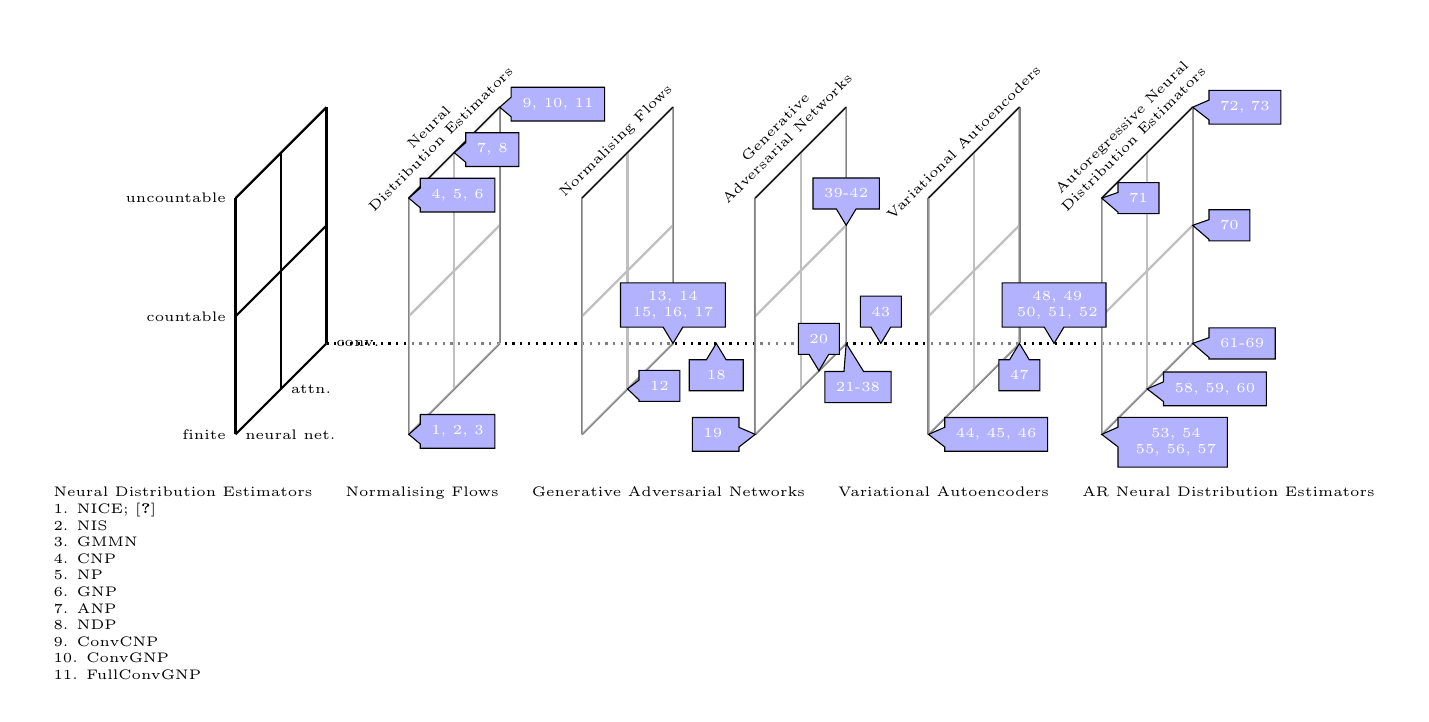
\begin{tikzpicture} %[tdplot_main_coords]
    
        % \pgfmathsetmacro{\d}{2.0}
        % \pgfmathsetmacro{\s}{1.3}
        % \tdplotsetrotatedcoords{10}{0}{0}
        
        % \draw[dotted, thick, red, tdplot_rotated_coords] (0, 0, 0) -- (1, 0, 0);
        % \draw[dotted, thick, green, tdplot_rotated_coords] (0, 0, 0) -- (0, 1, 0);
        % \draw[dotted, thick, blue, tdplot_rotated_coords] (0, 0, 0) -- (0, 0, 1);
    
        \pgfmathsetmacro{\d}{2.2}
        \pgfmathsetmacro{\s}{1.5}
        
        \draw[dotted, thick] (0, {-1*\s}, {-1*\s}) -- ({\d*5}, {-1*\s}, {-1*\s});
            
        \foreach \y in {-1,...,1}
        {
            \draw[thick, black] (0, {\y*\s}, {-1*\s}) -- (0, {\y*\s}, \s);
        }
            
        \foreach \z in {-1,...,1}
        {
            \draw[thick, black] (0, {-1*\s}, {\z*\s}) -- (0, \s, {\z*\s});
        }
        
        \foreach \x in {1,...,5}
        {
            
            \foreach \y in {-1,...,1}
            {
                \draw[thick, gray] ({\x*\d}, {\y*\s}, {-1*\s}) -- ({\x*\d}, {\y*\s}, \s);
            }
            
            \foreach \z in {-1,...,1}
            {
                \draw[thick, gray] ({\x*\d}, {-1*\s}, {\z*\s}) -- ({\x*\d}, \s, {\z*\s});
            }
            
            \draw[draw=gray, fill=white, opacity=0.5] ({\x*\d}, {-1*\s}, {-1*\s}) -- ({\x*\d}, {-1*\s}, \s) -- ({\x*\d}, \s, \s) -- ({\x*\d}, \s, {-1*\s}) -- cycle;
            
        }
        
        \draw (\d, \s, \s) -- (\d, \s, {-1*\s}) node [midway, above, sloped] (NDE) {\tiny \begin{tabular}{c} Neural \\ Distribution Estimators \end{tabular}};
        
        \draw (2*\d, \s, \s) -- (2*\d, \s, {-1*\s}) node [midway, above, sloped] (NF) {\tiny Normalising Flows};
        
        \draw (3*\d, \s, \s) -- (3*\d, \s, {-1*\s}) node [midway, above, sloped] (GAN) {\tiny \begin{tabular}{c} Generative \\ Adversarial Networks \end{tabular}};
        
        \draw (4*\d, \s, \s) -- (4*\d, \s, {-1*\s}) node [midway, above, sloped] (GAN) {\tiny Variational Autoencoders};
        
        \draw (5*\d, \s, \s) -- (5*\d, \s, {-1*\s}) node [midway, above, sloped] (NDE) {\tiny \begin{tabular}{c} Autoregressive Neural \\ Distribution Estimators \end{tabular}};
        
        \node at (\d, -\s, \s) (nfn) {};
        \node[rectangle callout,fill=blue!30,draw,inner sep = 4pt,callout absolute pointer={(nfn)},anchor=west] at ($(nfn) + (0.1, 0, -0.1)$) {\color{white} \tiny 1, 2, 3}; 
        
        \node at (\d, \s, \s) (nun) {};
        \node[rectangle callout,fill=blue!30,draw,inner sep = 4pt,callout absolute pointer={(nun)},anchor=west] at ($(nun) + (0.1, 0, -0.1)$) {\color{white} \tiny 4, 5, 6}; 
        
        \node at (\d, \s, 0) (aun) {};
        \node[rectangle callout,fill=blue!30,draw,inner sep = 4pt,callout absolute pointer={(aun)},anchor=west] at ($(aun) + (0.1, 0, -0.1)$) {\color{white} \tiny 7, 8}; 
        
        \node at (\d, \s, -\s) (cun) {};
        \node[rectangle callout,fill=blue!30,draw,inner sep = 4pt,callout absolute pointer={(cun)},anchor=west] at ($(cun) + (0.1, 0, -0.1)$) {\color{white} \tiny 9, 10, 11}; 
        
        \node at (2*\d, -\s, 0) (afn) {};
        \node[rectangle callout,fill=blue!30,draw,inner sep = 4pt,callout absolute pointer={(afn)},anchor=west] at ($(afn) + (0.1, 0, -0.1)$) {\color{white} \tiny 12}; 
        
        \node at (2*\d, -\s, -\s) (cfn) {};
        \node[rectangle callout,fill=blue!30,inner sep=2.0pt, draw,callout absolute pointer={(cfn)},anchor=south] at ($(cfn) + (0, 0.2, 0)$) {\color{white} \tiny \hspace*{-6pt} \begin{tabular}{c} 13, 14 \\ 15, 16, 17 \end{tabular} \hspace*{-6pt}}; 
        
        \node at (2.25*\d, -\s, -\s) (cfn2) {};
        \node[rectangle callout,fill=blue!30, draw,callout absolute pointer={(cfn2)},inner sep = 4pt,anchor=north] at ($(cfn2) + (0, -0.2, 0)$) {\color{white} \tiny ~18~~}; 
        
        \node at (3*\d, -\s, \s) (nfg) {};
        \node[rectangle callout,fill=blue!30, draw,callout absolute pointer={(nfg)},inner sep = 4pt,anchor=east] at ($(nfg) + (-0.2, 0, 0)$) {\color{white} \tiny 19\phantom{,}};
        
        \node at (3*\d, -\s, -0.4*\s) (nfg2) {};
        \node[rectangle callout,fill=blue!30, draw,callout absolute pointer={(nfg2)},inner sep = 4pt, anchor=south] at ($(nfg2) + (0, 0.2, 0)$) {\color{white} \tiny 20};
        
        \node at (3*\d, -\s, -\s) (cfg) {};
        \node[rectangle callout,fill=blue!30, inner sep = 4pt, draw,callout absolute pointer={(cfg)},anchor=north] at ($(cfg) + (0.15, -0.35, 0)$) {\color{white} \tiny 21-38};
        
        \node at (3*\d, 0, -\s) (ccg) {};
        \node[rectangle callout,fill=blue!30, draw,inner sep = 4pt,callout absolute pointer={(ccg)},anchor=south] at ($(ccg) + (0, 0.2, 0)$) {\color{white} \tiny 39-42};
        
        \node at (3.2*\d, -\s, -\s) (cfg2) {};
        \node[rectangle callout,fill=blue!30, inner sep = 4pt, draw,callout absolute pointer={(cfg2)},anchor=south] at ($(cfg2) + (0, 0.2, 0)$) {\color{white} \tiny 43};
        
        \node at (4*\d, -\s, \s) (nfv) {};
        \node[rectangle callout,fill=blue!30, inner sep = 4pt, draw,callout absolute pointer={(nfv)},anchor=west] at ($(nfv) + (0.2, 0, 0)$) {\color{white} \tiny 44, 45, 46};
        
        \node at (4*\d, -\s, -\s) (ccv) {};
        \node[rectangle callout,fill=blue!30, inner sep = 4pt, draw,callout absolute pointer={(ccv)},anchor=north] at ($(ccv) + (0, -0.2, 0)$) {\color{white} \tiny 47};
        
        \node at (4.2*\d, -\s, -\s) (ccv2) {};
        \node[rectangle callout,fill=blue!30, inner sep = 2.0pt, draw,callout absolute pointer={(ccv2)},anchor=south] at ($(ccv2) + (0, 0.2, 0)$) {\color{white} \tiny \hspace*{-5pt} \begin{tabular}{c} 48, 49 \\ 50, 51, 52 \end{tabular}\hspace*{-5pt}};
        
        \node at (5*\d, -\s, \s) (nfa) {};
        \node[rectangle callout,fill=blue!30, inner sep = 3.0pt, draw,callout absolute pointer={(nfa)},anchor=west] at ($(nfa) + (0.2, -0.1, 0)$) {\color{white} \tiny \hspace*{-5pt} \begin{tabular}{c} 53, 54 \\ 55, 56, 57 \end{tabular}\hspace*{-5pt}};
        
        \node at (5*\d, -\s, 0) (afa) {};
        \node[rectangle callout,fill=blue!30, inner sep = 4.0pt, draw,callout absolute pointer={(afa)},anchor=west] at ($(afa) + (0.2, 0, 0)$) {\color{white} \tiny 58, 59, 60};
        
        \node at (5*\d, -\s, -\s) (cfa) {};
        \node[rectangle callout,fill=blue!30, inner sep = 4.0pt, draw,callout absolute pointer={(cfa)},anchor=west] at ($(cfa) + (0.2, 0, 0)$) {\color{white} \tiny 61-69};
        
        \node at (5*\d, 0, -\s) (cca) {};
        \node[rectangle callout,fill=blue!30, inner sep = 4.0pt, draw,callout absolute pointer={(cca)},anchor=west] at ($(cca) + (0.2, 0, 0)$) {\color{white} \tiny 70};
        
        \node at (5*\d, \s, \s) (nua) {};
        \node[rectangle callout,fill=blue!30, inner sep = 4.0pt, draw,callout absolute pointer={(nua)},anchor=west] at ($(nua) + (0.2, 0, 0)$) {\color{white} \tiny 71};
        
        \node at (5*\d, \s, -\s) (cua) {};
        \node[rectangle callout,fill=blue!30, inner sep = 4.0pt, draw,callout absolute pointer={(cua)},anchor=west] at ($(cua) + (0.2, 0, 0)$) {\color{white} \tiny 72, 73};
        
        \node at (0, -\s, \s) (n0) {};
        \node[anchor=west] at ($(n0) + (0, 0, 0)$) {\tiny neural net.};
        
        \node at (0, -\s, 0) (a0) {};
        \node[anchor=west] at ($(a0) + (0, 0, 0)$) {\tiny attn.};
        
        \node at (0, -\s, -\s) (cv0) {};
        \node[anchor=west] at ($(cv0) + (0, 0, 0)$) {\tiny conv.};
        
        \node at (0, -\s, \s) (f0) {};
        \node[anchor=east] at ($(f0) + (0, 0, 0)$) {\tiny finite};
        
        \node at (0, 0, \s) (c0) {};
        \node[anchor=east] at ($(c0) + (0, 0, 0)$) {\tiny countable};
        
        \node at (0, \s, \s) (u0) {};
        \node[anchor=east] at ($(u0) + (0, 0, 0)$) {\tiny uncountable};
        
        \node at (2.5*\d, -2.6, 0.0) (u0) {};
        \node[anchor=north] at ($(u0) + (0, 0, 0)$) {\tiny \begin{tabular}{l l l l l}
            Neural Distribution Estimators &
            Normalising Flows & Generative Adversarial Networks & Variational Autoencoders & AR Neural Distribution Estimators \\
            1. NICE; \cite{dihn2014nice} & & & & \\
            2. NIS & & & & \\
            3. GMMN & & & & \\
            4. CNP & & & & \\
            5. NP & & & & \\
            6. GNP & & & & \\
            7. ANP & & & & \\
            8. NDP & & & & \\
            9. ConvCNP & & & & \\
            10. ConvGNP & & & & \\
            11. FullConvGNP & & & &
        \end{tabular}};
    

        % \pgfmathsetmacro{\d}{2.5}
        % \tdplotsetrotatedcoords{0}{0}{0}
        
        % \foreach \x in {-1,...,1}
        % {
        %     \draw[thick, black, tdplot_rotated_coords] (\x, -1, 0) -- (\x, 1, 0);
        % }
            
        % \foreach \y in {-1,...,1}
        % {
        %     \draw[thick, black, tdplot_rotated_coords] (-1, \y, 0) -- (1, \y, 0);
        % }
        
        % \foreach \z in {1,...,5}
        % {
            
        %     \foreach \x in {-1,...,1}
        %     {
        %         \draw[thick, gray, tdplot_rotated_coords] (\x, -1, {\z*\d}) -- (\x, 1, {\z*\d});
        %     }
            
        %     \foreach \y in {-1,...,1}
        %     {
        %         \draw[thick, gray, tdplot_rotated_coords] (-1, \y, {\z*\d}) -- (1, \y, {\z*\d});
        %     }
            
        %     \draw[draw=gray, fill=white, opacity=0.3, tdplot_rotated_coords] (-1, -1, {\z*\d}) -- (1, -1, {\z*\d}) -- (1, 1, {\z*\d}) -- (-1, 1, {\z*\d}) -- cycle;
            
        % }
        
        % \draw[dotted, thick, tdplot_rotated_coords] (1, -1, 0) -- (1, -1, {\d*5});
        
    \end{tikzpicture}
    
\bibliography{iclr2023_conference}

\end{document}